\documentclass[dvipdfmx,11pt]{beamer}

%全体設定
%\AtBeginDvi{\special{pdf:tounicode 90ms-RKSJ-UCS2}}
%%%%%%%%%%%%%%%%%%%%%%%%%%%%%%%%%%%%%%%%%%%%%%%%%%%%%%%%%%%%%%%%
% User-defined Macro
%%%%%%%%%%%%%%%%%%%%%%%%%%%%%%%%%%%%%%%%%%%%%%%%%%%%%%%%%%%%%%%%
\newcommand{\compress}{\itemsep0pt\parsep0pt\parskip0pt\partopsep0pt}
% \newcommand{\compress}{\itemsep1pt plus1pt\parsep0pt\parskip0pt}
% \newcommand{\code}[1]{\lstinline[basicstyle=\ttfamily]{#1}}
\newcommand{\gringo}{\textit{gringo}}
\newcommand{\clasp}{\textit{clasp}}
\newcommand{\clingo}{\textit{clingo}}
\newcommand{\teaspoon}{\textit{teaspoon}}
\newcommand{\sat}{\textsf{SAT}}
\newcommand{\unsat}{\textsf{UNSAT}}
% \newcommand{\web}[2]{\href{#1}{#2\ \raisebox{-0.15ex}{\beamergotobutton{Web}}}}
% \newcommand{\doi}[2]{\href{#1}{#2\ \raisebox{-0.15ex}{\beamergotobutton{DOI}}}}
% \newcommand{\weblink}[1]{\web{#1}{#1}}
% \newcommand{\imp}{\mathrel{\Rightarrow}}
% \newcommand{\Iff}{\mathrel{\Leftrightarrow}}
% \newcommand{\mybox}[1]{\fbox{\rule[.2cm]{0cm}{0cm}\mbox{${#1}$}}}
% \newcommand{\mycbox}[2]{\tikz[baseline]\node[fill=#1!10,anchor=base,rounded corners=2pt] () {#2};}
% \newcommand{\naf}[1]{\ensuremath{{\sim\!\!{#1}}}}
% \newcommand{\head}[1]{\ensuremath{\mathit{head}(#1)}}
% \newcommand{\body}[1]{\ensuremath{\mathit{body}(#1)}}
% \newcommand{\atom}[1]{\ensuremath{\mathit{atom}(#1)}}
% \newcommand{\poslits}[1]{\ensuremath{{#1}^+}}
% \newcommand{\neglits}[1]{\ensuremath{{#1}^-}}
% \newcommand{\pbody}[1]{\poslits{\body{#1}}}
% \newcommand{\nbody}[1]{\neglits{\body{#1}}}
% \newcommand{\Cn}[1]{\ensuremath{\mathit{Cn}(#1)}}
% \newcommand{\reduct}[2]{\ensuremath{#1^{#2}}}
% \newcommand{\OK}{\mbox{\textcolor{green}{\Pisymbol{pzd}{52}}}}
% \newcommand{\KO}{\mbox{\textcolor{red}{\Pisymbol{pzd}{56}}}}
% \newcommand{\code}[1]{\lstinline[basicstyle=\ttfamily]{#1}}
% \newcommand{\lw}[1]{\smash{\lower2.ex\hbox{#1}}}
\newcommand{\llw}[1]{\smash{\lower3.ex\hbox{#1}}}

\newenvironment{tableC}{%
  \scriptsize
  \renewcommand{\arraystretch}{0.9}
  \tabcolsep = 0.6mm
  % \begin{tabular}[t]{p{6mm}|rlr|rlr|rlr|rlr|rlr}\hline
  %   \multicolumn{1}{l|}{\llw{問題   }} &
  \begin{tabular}[t]{l|rlr|rlr|rlr|rlr|rlr}\hline
    \multicolumn{1}{l|}{\llw{問題}} &
    \multicolumn{3}{c|}{UD1} &
    \multicolumn{3}{c|}{UD2} &
    \multicolumn{3}{c|}{UD3} &
    \multicolumn{3}{c|}{UD4} &
    \multicolumn{3}{c}{UD5} \\
    & 
    \multicolumn{1}{c}{既知の} & & \multicolumn{1}{c|}{ASP} & 
    \multicolumn{1}{c}{既知の} & & \multicolumn{1}{c|}{ASP} & 
    \multicolumn{1}{c}{既知の} & & \multicolumn{1}{c|}{ASP} & 
    \multicolumn{1}{c}{既知の} & & \multicolumn{1}{c|}{ASP} & 
    \multicolumn{1}{c}{既知の} & & \multicolumn{1}{c}{ASP} \\
    & 
    ベスト & &  & 
    ベスト & &  & 
    ベスト & &  & 
    ベスト & &  & 
    ベスト & &  \\
    \hline
  }{%
    \hline
  \end{tabular}
}

%\usetheme{Madrid}

\title[ASPを用いた組合せ遷移問題の解法に関する考察]{解集合プログラミングを用いた\\組合せ遷移問題の解法に関する考察}
\author{252105205~~~山田~悠也}
\date{2021年度番原研研究紹介\\2021年4月23日}
\institute{番原研究室}

%% テンプレ 
\begin{comment}

%%%%%%%%%%%%%%%%%%%%%%%%%%%%%%%%%%%%%%%%%%%%%%%%%%
%% タイトル
%%%%%%%%%%%%%%%%%%%%%%%%%%%%%%%%%%%%%%%%%%%%%%%%%%
\begin{frame}\frametitle{}
\end{frame}

\end{comment}

%###########################################################
%# 本文 ####################################################
%###########################################################
\begin{document}

%%%%%%%%%%%%%%%%%%%%%%%%%%%%%%%%%%%%%%%%%%%%%%%%%%
%% タイトル 
%%%%%%%%%%%%%%%%%%%%%%%%%%%%%%%%%%%%%%%%%%%%%%%%%%
\begin{frame}\frametitle{}
  \titlepage
\end{frame}

%%%%%%%%%%%%%%%%%%%%%%%%%%%%%%%%%%%%%%%%%%%%%%%%%%
%% 組合せ遷移問題
%%%%%%%%%%%%%%%%%%%%%%%%%%%%%%%%%%%%%%%%%%%%%%%%%%
\begin{frame}\frametitle{組合せ遷移問題(Combinatorial Reconfiguration Problems)}

  \begin{alertblock}{}
    \alert{\bf 組合せ遷移問題}とは,
    基となる組合せ問題とその二つの実行可能解が与えられたとき,一方の実行可能解
    から他方の実行可能解へ,遷移制約を満たしつつ,
    実行可能解のみを経由して到達できるかを判定する問題.
  \end{alertblock}

  \begin{itemize}
    %\item 既存の組合せ問題の多くを組合せ遷移問題に拡張できる.
    \item 基となる問題が NP 完全である場合,その遷移問題の多くは,
      \alert{PSPACE完全}であることが知られている~[伊藤 '18].
    %\item \structure{持続可能なシステム}への応用が期待されている.
    \item 理論的な基盤が整備されつつある一方で,
      組合せ遷移問題の\alert{汎用的かつ効率的なアルゴリズムは見つかっていない}.
    \item 代表的な組合せ遷移問題
      \begin{itemize}
      \item 命題論理の充足可能性判定問題(SAT)の遷移問題~[Gopalan+ '09]
      \item 集合被覆問題の遷移問題~[Ito+ '11]
      \item グラフ点彩色問題の遷移問題~[Paul Bonsma+ '09]
      \end{itemize}
  \end{itemize}

  \pause
  \begin{alertblock}{}\centering
    本研究では,グラフ点彩色問題の遷移問題(\alert{$k$彩色遷移問
      題})を扱う.
  \end{alertblock}

  
\end{frame}

%%%%%%%%%%%%%%%%%%%%%%%%%%%%%%%%%%%%%%%%%%%%%%%%%%
%% k彩色遷移問題
%%%%%%%%%%%%%%%%%%%%%%%%%%%%%%%%%%%%%%%%%%%%%%%%%%
\begin{frame}\frametitle{$k$彩色遷移問題}

  \begin{block}{$k$彩色遷移問題}
    \begin{itemize}
    \item 問題の入力は,グラフ点彩色問題とその二つの実行可能解
      \structure{$\alpha$}(初期状態)と\structure{$\beta$}(目標状態).
    \item $\alpha$から$\beta$への到達可能性を判定することが目的.
    \item \structure{各遷移で色が変化する頂点はただ一つのみ} (遷移制約).
    \end{itemize}
  \end{block}

  \begin{exampleblock}{$k$彩色遷移問題の例}
    \begin{columns}
      \begin{column}{0.3\textwidth}
        \centering
        \begin{tikzpicture}
 \draw (0,0)--(8,0);
 \draw (0,1)--(8,1);
 \draw (0,2)--(8,2);
 \draw (0,3)--(8,3);
 \draw (0,4)--(8,4);
 \draw (0,5)--(8,5);
 \draw (0,6)--(8,6);
 \draw (0,7)--(8,7);
 \draw (0,8)--(8,8);
 \draw (0,0)--(0,8);
 \draw (1,0)--(1,8);
 \draw (2,0)--(2,8);
 \draw (3,0)--(3,8);
 \draw (4,0)--(4,8);
 \draw (5,0)--(5,8);
 \draw (6,0)--(6,8);
 \draw (7,0)--(7,8);
 \draw (8,0)--(8,8);
 \draw (0,0)--(0,8);
 %\fill[red] (4.5,7.5) circle (0.3);
 \draw[red] (4.5,0.5)--(4.5,7.5);
 \draw[red] (0.5,7.5)--(7.5,7.5);
 \draw[red] (0.5,3.5)--(4.5,7.5);
 \draw[red] (7.5,4.5)--(4.5,7.5);
 %\fill[cyan] (6.5,6.5) circle (0.3);
 \draw[cyan] (0.5,6.5)--(7.5,6.5);
 \draw[cyan] (6.5,0.5)--(6.5,7.5);
 \draw[cyan] (0.5,0.5)--(7.5,7.5);
 \draw[cyan] (5.5,7.5)--(7.5,5.5);
 %\fill[violet] (0.5,3.5) circle (0.3);
 \draw[violet] (0.5,3.5)--(7.5,3.5);
 \draw[violet] (0.5,0.5)--(0.5,7.5);
 \draw[violet] (0.5,3.5)--(4.5,7.5);
 \draw[violet] (0.5,3.5)--(3.5,0.5);
 %\fill[teal] (3.5,2.5) circle (0.3);
 \draw[teal] (0.5,2.5)--(7.5,2.5);
 \draw[teal] (3.5,0.5)--(3.5,7.5);
 \draw[teal] (1.5,0.5)--(7.5,6.5);
 \draw[teal] (0.5,5.5)--(5.5,0.5);
 %\fill[orange] (6.5,0.5) circle (0.3);
 \draw[orange] (0.5,0.5)--(7.5,0.5);
 \draw[orange] (6.5,0.5)--(6.5,7.5);
 \draw[orange] (6.5,0.5)--(0.5,6.5);
 \draw[orange] (6.5,0.5)--(7.5,1.5);
 \fill[red] (4.5,7.5) \symqueen ;
 \fill[cyan] (6.5,6.5) circle (0.35);
 \fill[violet] (0.5,3.5) circle (0.35);
 \fill[teal] (3.5,2.5) circle (0.35);
 \fill[orange] (6.5,0.5) circle (0.35);
\end{tikzpicture}
        ステップ0($=\alpha$)
      \end{column}
      \begin{column}{0.05\textwidth}
        \textbf{$\longrightarrow$}
      \end{column}
      \begin{column}[]{0.3\textwidth}
        \centering
        %%%%%%%%%%%%%%%%%%%%%%%%%%%%%%%%%%%%%%%%%%%%%%%%%%
% 実行例(t=0) (第6章で使う)
%%%%%%%%%%%%%%%%%%%%%%%%%%%%%%%%%%%%%%%%%%%%%%%%%%

\begin{tikzpicture}[scale=0.6]

  % 設定
  \tikzset{node/.style={circle,draw=black}}
 
  \definecolor{col_r}{RGB}{230,0,18}
  %\definecolor{col_b}{RGB}{0,104,183}
  \definecolor{col_b}{RGB}{51,51,179}
  \definecolor{col_y}{RGB}{255,251,0}
  \definecolor{col_g}{RGB}{0,96,0}
 
  % 補助線
  % \draw [help lines,blue] (0,0) grid (20,6);
 
  % node %
  \node[node, fill=col_y!70] (node1){\textbf{1}};
  \node[node, fill=col_b!70, right=of node1] (node2){\textbf{2}};
  \node[node, fill=col_y!70, below=of node1] (node3){\textbf{3}};
  \node[node, fill=col_g!70, below=of node2] (node4){\textbf{4}};
 
  \foreach \u / \v in {node1/node2, node2/node3, node2/node4, node3/node4}
  \draw (\u) -- (\v);
 \end{tikzpicture}
 
 %%%%%%%%%%%%%%%%%%%%%%%%%%%%%%%%%%%%%%%%%%%%%%%%%%%%%%%%%%
 %%% Local Variables:
 %%% mode: japanese-latex
 %%% TeX-master: paper.tex
 %%% End:
 
        ステップ1
      \end{column}
      \begin{column}{0.05\textwidth}
        \textbf{$\longrightarrow$}
      \end{column}
      \begin{column}{0.3\textwidth}
        \centering
        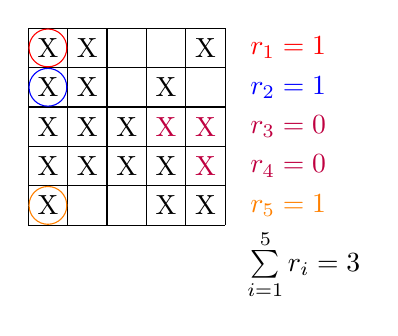
\begin{tikzpicture}
 \draw (0,0)--(2.5,0);
 \draw (0,0.5)--(2.5,0.5);
 \draw (0,1.0)--(2.5,1.0);
 \draw (0,1.5)--(2.5,1.5);
 \draw (0,2.0)--(2.5,2.0);
 \draw (0,2.5)--(2.5,2.5);
 \draw (0,0)--(0,2.5);
 \draw (0.5,0)--(0.5,2.5);
 \draw (1.0,0)--(1.0,2.5);
 \draw (1.5,0)--(1.5,2.5);
 \draw (2.0,0)--(2.0,2.5);
 \draw (2.5,0)--(2.5,2.5);
 \node (X) at (0.25,0.25) {X};
 \draw [orange] (0.25,0.25) circle[radius = 0.24];
 \node (X) at (0.25,0.75) {X};
 \node (X) at (0.25,1.25) {X};
 \node (X) at (0.25,1.75) {X};
 \draw [blue] (0.25,1.75) circle[radius = 0.24];
 \node (X) at (0.25,2.25) {X};
 \draw [red] (0.25,2.25) circle[radius = 0.24];
 \node (X) at (0.75,2.25) {X};
 \node (X) at (0.75,0.75) {X};
 \node (X) at (0.75,1.25) {X};
 \node (X) at (0.75,1.75) {X};
 \node (X) at (1.25,0.75) {X};
 \node (X) at (1.25,1.25) {X};
 \node (X) at (1.75,0.25) {X};
 \node (X) at (1.75,0.75) {X};
 \node (X) at (1.75,1.25) {\color{purple}X};
 \node (X) at (1.75,1.75) {X};
 \node (X) at (2.25,0.25) {X};
 \node (X) at (2.25,0.75) {\color{purple}X};
 \node (X) at (2.25,1.25) {\color{purple}X};
 \node (X) at (2.25,2.25) {X};
 \node (A) at (3.30,2.25) {\color{red}$r_{1} = 1$};
 \node (B) at (3.30,1.75) {\color{blue}$r_{2} = 1$};
 \node (M) at (3.30,1.25) {\color{purple}$r_{3} = 0$};
 \node (M) at (3.30,0.75) {\color{purple}$r_{4} = 0$};
 \node (C) at (3.30,0.25) {\color{orange}$r_{5} = 1$};
 \node (D) at (3.50,-0.50) {$\sum\limits_{i=1}^{5}r_{i}=3$};
\end{tikzpicture}
        ステップ2($=\beta$)
      \end{column}
    \end{columns}
  \end{exampleblock}
  
\end{frame}
%%%%%%%%%%%%%%%%%%%%%%%%%%%%%%%%%%%%%%%%%%%%%%%%%%
%% ASP
%%%%%%%%%%%%%%%%%%%%%%%%%%%%%%%%%%%%%%%%%%%%%%%%%%

\begin{frame}\frametitle{解集合プログラミング(Answer Set Programming; ASP)}

  \begin{itemize}
    \item ASP言語は一階論理に基づいた知識表現言語の一種である.
    \item ASPシステムは安定モデル理論~[Gelfond and Lifschitz '88] に基づく
          解集合を計算するシステムである.
    \item 近年,SAT技術の応用により高速なASPシステムが実現し, 
          システム検証やプランニングなどの様々な分野での実用的応用が拡大している.
  \end{itemize}

  \begin{alertblock}{組合せ遷移問題に対してASPを用いる利点}
    \begin{itemize}
      \item ASPの高い表現力により,記号制約を簡潔に記述できる.
      \item インクリメンタルASP解法により,同様の探索失敗を避けるために獲得した学習節を保持することで,遷移問題に対する効率的な解探索が可能である.
    \end{itemize}
  \end{alertblock}
  
\end{frame}

%%%%%%%%%%%%%%%%%%%%%%%%%%%%%%%%%%%%%%%%%%%%%%%%%%
%% 研究目的
%%%%%%%%%%%%%%%%%%%%%%%%%%%%%%%%%%%%%%%%%%%%%%%%%%

\begin{frame}\frametitle{研究目的}
  \begin{alertblock}{目的}
    ASP技術を活用し,大規模な組合せ遷移問題を効率よく解くシステムを実現する.%組合せ遷移問題の一つであり,PSPACE完全な問題の一つでもある$k \ge 4$の$k$彩色遷移問題を高速で解く.%ける符号化を提案し評価する.
  \end{alertblock}
  \begin{itemize}
  \item 本発表では,$k$彩色遷移問題を対象とする.
  \end{itemize}
  \begin{block}{研究内容}
    \begin{enumerate}
    \item $k$彩色遷移問題を解く,3種類の ASP 符号化を提案した.
    \item \textit{COLOR04}~\footnotemark[1]
      で公開されているグラフ点彩色問題をベースに,$k$彩色遷移問題のベ
      ンチマーク問題を新たに90問作成した.
    \item 独自に作成したベンチマーク問題を用い,3種のASP符号化の評価実験を行った.
    \end{enumerate}
  \end{block}
\footnotetext[1]{\url{https://mat.tepper.cmu.edu/COLOR04/}}  
\end{frame}

%%%%%%%%%%%%%%%%%%%%%%%%%%%%%%%%%%%%%%%%%%%%%%%%%%
%% 符号化
%%%%%%%%%%%%%%%%%%%%%%%%%%%%%%%%%%%%%%%%%%%%%%%%%%

\begin{frame}\frametitle{提案する$k$彩色遷移問題のASP符号化}

  \begin{block}{}\centering
    $k$彩色遷移問題を解く3種類のASP符号化,\\origin, changed, unchanged を考案.
  \end{block}

  \begin{itemize}
  \item 各符号化は,
    \structure{「各遷移で色が変化する頂点はただ一つのみ」}という遷
    移制約の表現方法が異なる.
  \item 表中の$|V|$は,グラフの頂点数を表す.
  \end{itemize}

  \begin{exampleblock}{}\centering
    \begin{tabular}{l|p{8cm}}
  符号化名 & 遷移制約 \\\hline
  origin & 任意の二つの頂点に対し違反する組合せを列挙することで表現  \\ \hline
  changed & 遷移制約を ASP の個数制約を用いて表現\\\hline
  unchanged & 「各遷移で色が変化しない頂点は$|V|-1$個」という制約を,
         ASPの個数制約を用いて表現
\end{tabular}
  \end{exampleblock}

  % \begin{table}
  %   \centering
  %   \begin{tabular}{l|p{8cm}}
  符号化名 & 遷移制約 \\\hline
  origin & 任意の二つの頂点に対し違反する組合せを列挙することで表現  \\ \hline
  changed & 遷移制約を ASP の個数制約を用いて表現\\\hline
  unchanged & 「各遷移で色が変化しない頂点は$|V|-1$個」という制約を,
         ASPの個数制約を用いて表現
\end{tabular}
  % \end{table}

  \begin{itemize}
  \item 特に,unchanged符号化は基礎化後の ASP のルール数を抑えるように工夫
    されており,大規模な問題に対する有効性が期待できる.
    \begin{itemize}
      \item 基礎化とは,一階述語論理に代入を行い命題論理へと変換すること.
    \end{itemize}
  \end{itemize}

\end{frame}

%%%%%%%%%%%%%%%%%%%%%%%%%%%%%%%%%%%%%%%%%%%%%%%%%%
%% ベンチマーク
%%%%%%%%%%%%%%%%%%%%%%%%%%%%%%%%%%%%%%%%%%%%%%%%%%
\begin{comment}
\begin{frame}\frametitle{ベンチマーク}

  \begin{itemize}
    \item 現時点で組合せ遷移問題は理論面の研究が主流であり, ベンチマークの整備が必要.
    \item 実験においてステップ$t$を与えるとき, その上限値が必要となる.
    \item ステップ$t$の上限値は, グラフ$G$を$k$彩色するときの実行可能解の数と等しい.
  \end{itemize}

  従って, 全解列挙が可能な($G, k$)からベンチマークを生成する必要がある.
  
\end{frame}
\end{comment}
%%%%%%%%%%%%%%%%%%%%%%%%%%%%%%%%%%%%%%%%%%%%%%%%%%
%% 実験環境
%%%%%%%%%%%%%%%%%%%%%%%%%%%%%%%%%%%%%%%%%%%%%%%%%%

\begin{frame}\frametitle{実験概要}
  提案した3種のASP符号化の評価にあたり,以下の実験を行った.
  \bigskip
  \begin{itemize}
    \item \structure{ベンチマーク問題}: 独自に作成した$k$彩色遷移問題(90問)
      \begin{enumerate}
      \item \textit{COLOR04}で公開されているグラフ点彩色問題のグラフ127個のうち,
      彩色数が判明している44個~[Tamura+ '09] をベンチマーク問題の候補とした.
      \item 44個のグラフに対して,彩色数での実行可能解を全列挙することが可能
            かを調査した.
      \item 総数を求められた9個のグラフから各10問ずつ,計90問のベンチマーク問題を作成した.
      \end{enumerate}
      % \begin{itemize}
      % \item \textit{COLOR04}で公開されている,グラフ点彩色問題Instances}に属するグラフから抜粋した9個を使用.
      % \item 各グラフ10問ずつベンチマークを作成.
      % \end{itemize}
%    \item \structure{色数}: 各グラフにおける彩色数

    \item \structure{ASPシステム}: \textit{clingo-5.4.0} \textit{jumpy}
    \item \structure{制限時間}: 3600秒/問
    \item \structure{環境}: Mac mini,3.2GHz 6コア Intel Core i7,64GB メモリ
  \end{itemize}
  
\end{frame}

%%%%%%%%%%%%%%%%%%%%%%%%%%%%%%%%%%%%%%%%%%%%%%%%%%
%% グラフの全解数
%%%%%%%%%%%%%%%%%%%%%%%%%%%%%%%%%%%%%%%%%%%%%%%%%%

\begin{frame}{独自に生成した$k$彩色遷移問題のベンチマーク問題}

  \begin{table}[t]
    \centering
    \begin{tabular}{lrrr|r}
  グラフ名 & 頂点数 & 辺数 & 彩色数 & 実行可能解の総数 \\ \hline
  1-FullIns\_3 & 30 & 100 & 4 & 50,693,280 \\ 
  le450\_5a & 450 & 5,714 & 5 & 3,840 \\ 
  le450\_5c & 450 & 9,803 & 5 & 120 \\ 
  le450\_5d & 450 & 9,757 & 5 & 960 \\ 
  myciel3 & 11 & 20 & 4 & 12,480 \\ 
  myciel4 & 23 & 71 & 5 & 2,845,658,400 \\ 
  queen5\_5 & 25 & 160 & 5 & 240 \\  
  queen6\_6 & 36 & 290 & 7 & 100,800 \\ 
  queen7\_7 & 49 & 476 & 7 & 20,160 \\
\end{tabular}
  \end{table}

  \begin{itemize}
  \item 彩色数とは,各グラフを彩色可能な最小の色数を意味する.
  \item 実行可能解の総数は,最少で120個,最大で約28億個である.
  \item 求められた実行可能解から解をランダムで二つ選びベンチマーク問題を作成し,
        各グラフから10問,計90問を作成した.
  \end{itemize}

\end{frame}

%%%%%%%%%%%%%%%%%%%%%%%%%%%%%%%%%%%%%%%%%%%%%%%%%%
%% 実験結果
%%%%%%%%%%%%%%%%%%%%%%%%%%%%%%%%%%%%%%%%%%%%%%%%%%

\begin{frame}\frametitle{実験結果: 解けた問題数}

提案符号化で解けた問題数は,以下の通りである.
\bigskip

\begin{exampleblock}{}\centering
  \begin{tabular}{l|rr|rr} 
  & \multicolumn{2}{c|}{基本ソルバー} & \multicolumn{2}{c}{改良ソルバー} \\
  & \code{changed} & \code{unchanged} & \code{changed} & \code{unchanged} \\ \hline
  解けた問題数(到達可能) & 11 & 11 & 11 & 11 \\
  解けた問題数(到達不能) & 10 & 10 & 56 & \alert{60} \\\hline
  平均 CPU 時間(秒) & 223.796 & 151.341 & 101.758 & \alert{59.095} \\
\end{tabular}
\end{exampleblock}

  % \begin{table}[t]
  %   \centering
  %   \begin{tabular}{l|rr|rr} 
  & \multicolumn{2}{c|}{基本ソルバー} & \multicolumn{2}{c}{改良ソルバー} \\
  & \code{changed} & \code{unchanged} & \code{changed} & \code{unchanged} \\ \hline
  解けた問題数(到達可能) & 11 & 11 & 11 & 11 \\
  解けた問題数(到達不能) & 10 & 10 & 56 & \alert{60} \\\hline
  平均 CPU 時間(秒) & 223.796 & 151.341 & 101.758 & \alert{59.095} \\
\end{tabular}
  % \end{table}
  
  \begin{itemize}
    \item 到達可能は時間内に解が見つかったことを意味する.
    \item 到達不能は時間内に解が存在しないと確かめられたことを意味する.
    \item 本発表では到達可能インスタンスの結果を紹介する.
  \end{itemize}

\end{frame}

%%%%%%%%%%%%%%%%%%%%%%%%%%%%%%%%%%%%%%%%%%%%%%%%%%
%% 実験結果
%%%%%%%%%%%%%%%%%%%%%%%%%%%%%%%%%%%%%%%%%%%%%%%%%%
\begin{frame}\frametitle{実験結果: 到達可能インスタンスにおけるCPU時間}

  \begin{table}[t]
    \centering
    \scalebox{0.8}{
\begin{tabular}{lrr|rrrr} \hline
  インスタンス & 頂点数 & 辺数 & 遷移回数 & vrc1 & vrc2 & vrc3 \\ \hline
  1-FullIns\_3\_col4\_1 & 30 & 100 & 11 & 47.394 & 1.367 & \textcolor{red}{1.059} \\ 
  myciel3\_col4\_1 & 11 & 20 & 11 & 2.450 & 0.180 & \textcolor{red}{0.150} \\ 
  myciel3\_col4\_3 & 11 & 20 & 11 & 2.611 & 0.206 & \textcolor{red}{0.153} \\ 
  myciel3\_col4\_4 & 11 & 20 & 13 & 4.717 & 0.487 & \textcolor{red}{0.442} \\ 
  myciel3\_col4\_7 & 11 & 20 & 8 & 0.970 & 0.090 & \textcolor{red}{0.072} \\ 
  myciel3\_col4\_8 & 11 & 20 & 9 & 1.419 & 0.119 & \textcolor{red}{0.092} \\ 
  myciel4\_col5\_2 & 23 & 71 & 16 & 763.484 & \textcolor{red}{42.717} & 49.151 \\ 
  myciel4\_col5\_3 & 23 & 71 & 14 & 358.494 & \textcolor{red}{17.103} & 21.239 \\ 
  myciel4\_col5\_4 & 23 & 71 & 7 & 26.987 & 0.256 & \textcolor{red}{0.192} \\ 
  myciel4\_col5\_6 & 23 & 71 & 10 & 102.396 & 1.524 & \textcolor{red}{1.391} \\ 
  myciel4\_col5\_10 & 23 & 71 & 17 & 818.589 & 212.066 & \textcolor{red}{73.48} \\ \hline
  Sum &  &  &  & 0 & 2 & 9 \\ \hline
\end{tabular}
}  
  \end{table}

  \begin{itemize}
    \item unchanged符号化は,最速であったインスタンスの数・総CPU時間の両方で優位性を示した.
  \end{itemize}
  
\end{frame}

%%%%%%%%%%%%%%%%%%%%%%%%%%%%%%%%%%%%%%%%%%%%%%%%%%
%% 今後の課題
%%%%%%%%%%%%%%%%%%%%%%%%%%%%%%%%%%%%%%%%%%%%%%%%%%

\begin{frame}\frametitle{まとめと今後の課題}

  \begin{block}{まとめ}
    \begin{itemize}
      \item $k$彩色遷移問題に対して,3種類の符号化を提案した.
      \begin{itemize}
      \item ASP の高い表現力を生かして,$k$彩色遷移問題を簡潔に記述.
      \item 特に,unchanged符号化は基礎化後のルール数を抑える工夫をしている.
      \end{itemize}
    \item \textit{COLOR04}
      で公開されているグラフ点彩色問題をベースに,$k$彩色遷移問題のベ
      ンチマーク問題を新たに90問作成した.
      % \begin{itemize}
      %   \item 実行可能解の総数が異なる問題から作成した.
      % \end{itemize}
    \item 独自に作成したベンチマーク問題を用い,3種のASP符号化の評価実験を行った.
      \begin{itemize}
      \item unchanged符号化の優位性が確かめられた.
      \end{itemize}
    \end{itemize}
  \end{block}
  
  \begin{alertblock}{今後の課題}
    \begin{itemize}
      \item インクリメンタル ASP 解法を用いた高速化.
      \item 他の組合せ遷移問題の符号化.
      \item ベンチマーク問題の充実.
    \end{itemize}
  \end{alertblock}

\end{frame}

%###########################################################
%##### 補助スライド ########################################
%###########################################################

%%%% 補助スライド

\begin{frame}{~}
 \centering
 - 補足用 -
\end{frame} 

\begin{frame}{補足 : スマートグリッド}
 \begin{itemize}
  \item \structure{スマートグリッド}とは,電力の供給側,需要側において双方向の
		やり取りを可能にする次世代の\structure{賢い}電力網である.
  \item 従来と違い,通信技術の発達により,使用状況などを
		リアルタイムに把握することが可能となった.
  \item その時に応じた最適な配電網を構成し,制御するといったことが考えられている.
		\begin{itemize}
		 \item 電力需要の変化による,配電ロスの少ない構成.
		 \item 自然エネルギーによる発電量の変動を補う構成.
		\end{itemize}
  \item ASP言語の表現力や拡張性が,こうした条件の追加に活用できる可能性がある.
 \end{itemize}
\end{frame}

%%%%%%%%%%%%%%%%%%%%%%%%%%%%%%%%%%%%%%%%%%%%%%%%%%
%% 電気制約
%%%%%%%%%%%%%%%%%%%%%%%%%%%%%%%%%%%%%%%%%%%%%%%%%%
\begin{frame}{補足 : 電気制約}
 \begin{itemize}
  \item \alert{電気制約}は,送電する電流$\cdot$電圧の適正範囲を保証する制約.
  \begin{itemize}
   \item 供給経路の各区間で許容電流を超えない.
   \item 電気抵抗による電圧降下が許容範囲を超えない.
   \item etc.
  \end{itemize}
  \item 電流と電圧が影響し合う\structure{実数ドメイン上の制約}によって表される.
		% \begin{itemize}
		%  		 \item 送電システム上の条件など.
		% \end{itemize}
  \item 実数ドメイン上の制約は,純粋なASPのみで扱うのは\alert{困難}.
		\begin{itemize}
		 \item 緩和問題として,変電所から供給できる家庭の数に上限をつける.
		 \item ASPMT技術により,ASPで得られた解について,
			   背景理論ソルバーと連携して実数ドメイン上の制約を調べる.
		\end{itemize}
 \end{itemize}
\end{frame}


%%%%%%%%%%%%%%%%%%%%%%%%%%%%%%%%%%%%%%%%%%%%%%%%%%
%% 基礎化
%%%%%%%%%%%%%%%%%%%%%%%%%%%%%%%%%%%%%%%%%%%%%%%%%%
\begin{frame}{補足 : ASPシステム}
 
 \vspace{-0.5cm}

 \begin{figure}[htbp]
  \centering
  %%%%%%%%%%%%%%%%%%%%%%%%%%%%%%%%%%%%%%%%%%%%%%%%%%
%% 基礎化の流れの図
%%%%%%%%%%%%%%%%%%%%%%%%%%%%%%%%%%%%%%%%%%%%%%%%%%
\begin{tikzpicture}

 \definecolor{edge}{RGB}{38,38,134}
 \definecolor{node}{RGB}{220,220,249}

 \definecolor{alert_edge}{RGB}{191,0,0}
 \definecolor{alert_node}{RGB}{249,200,200}

 \definecolor{ex_edge}{RGB}{0,96,0}
 \definecolor{ex_node}{RGB}{230,239,230}

 \def\nodespace{2.4cm}

 \tikzset{block/.style={rectangle, thick, draw=edge, fill=node, text width=3cm, 
 text centered, rounded corners, text width=2cm, minimum height=1.5cm}};

 \tikzset{alertblock/.style={rectangle, thick, draw=alert_edge, fill=alert_node, 
 text width=3cm, text centered, rounded corners, text width=1.5cm, minimum height=1.2cm}};

 \node[block](ikkai){一階ASP\\プログラム};

 \node[rectangle,rounded corners, thick, draw=ex_edge, fill=ex_node, 
 right=0.22*\nodespace of ikkai, minimum width=6cm, minimum height=3cm, 
 text centered, label=ASPシステム](sys){};

 \node[block, right=\nodespace of ikkai](meidai){命題ASP\\プログラム};
 \node[block, right=\nodespace of meidai](ASP){解集合};

 \node[right=0.6*\nodespace of ikkai, text width=1.5cm, 
 text centered, text=red, anchor=south](){基礎化\\ソルバー};
 \node[right=0.4*\nodespace of meidai, text width=1.5cm, 
 text centered, text=red, anchor=south](){解集合\\ソルバー};

 
 \foreach \u / \v / \n in {ikkai/meidai,meidai/ASP}
 \draw [thick,->] (\u) to (\v);

\end{tikzpicture}
 \end{figure}

 \vspace{-0.5cm}

 \begin{exampleblock}{}
  \begin{enumerate}
   \item 一階ASPプログラムを基礎化ソルバーによって,
		 命題ASPプログラムに\alert{基礎化}する.
   \item 命題ASPプログラムについて,SAT技術を応用した解集合ソルバーが解集合を探索する.
  \end{enumerate}
 \end{exampleblock}

\end{frame}


%%%%%%%%%%%%%%%%%%%%%%%%%%%%%%%%%%%%%%%%%%%%%%%%%%
%% ASPのコード
%%%%%%%%%%%%%%%%%%%%%%%%%%%%%%%%%%%%%%%%%%%%%%%%%%
\begin{frame}[fragile]{補足 : 基本符号化のASPプログラム}
 \begin{exampleblock}{}
  \begin{center}
   %%%%%%%%%%%%%%%%%%%%%%%%%%%%%%%%%
   \lstinputlisting[numbers=left,%
   basicstyle=\ttfamily\tiny]{code/srf1.lp}
   %%%%%%%%%%%%%%%%%%%%%%%%%%%%%%%%% 
  \end{center}
 \end{exampleblock}
\end{frame}

\begin{frame}[fragile]{補足 : 改良符号化のASPプログラム}

 \begin{exampleblock}{}
  \begin{center}
   %%%%%%%%%%%%%%%%%%%%%%%%%%%%%%%%%
   \lstinputlisting[numbers=left,%
   basicstyle=\ttfamily\tiny]{code/srf2.lp}
   %%%%%%%%%%%%%%%%%%%%%%%%%%%%%%%%% 
  \end{center}
 \end{exampleblock}

\end{frame}



\end{document}